\begin{solutionfigure}[htb]
    \centering
    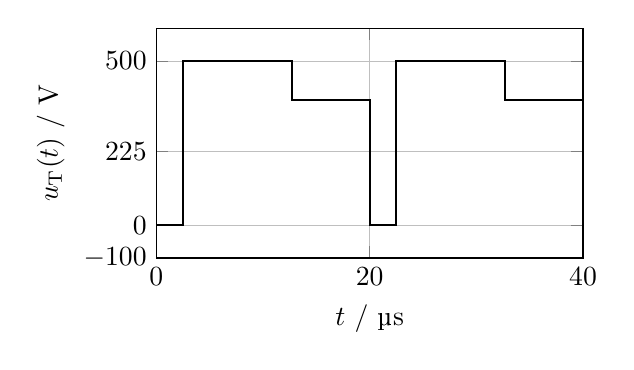
\begin{tikzpicture}
    \begin{axis}[
        width=7cm, height=4.5cm,
        grid=both,
        major grid style={line width=.2pt,draw=gray!50},
        minor grid style={line width=.1pt,draw=gray!20},
        xlabel={$t$ / µs},
        ylabel={$u_\mathrm{T}(t)$ / V},
       % title={$i_\mathrm{L}$ for minimum output power},
        xmin=0, xmax=40,
        ymin=-100, ymax=600,
        xtick={0, 20, 40},
        ytick={-100, 0, 225, 500},
        ]
        % Einschaltverhalten graph
        \addplot[
            thick,
            mark=none,
            color=black,
        ] coordinates {
            (0,0) (2.5,0) (2.5, 500) (12.7, 500) (12.7, 382) (20, 382) (20, 0) (22.5, 0)(22.5, 500) (32.7, 500) (32.7, 382) (40, 382)
        };
    \end{axis}
    \end{tikzpicture} 
    \hspace{1cm} % Abstand zwischen den beiden Diagrammen
    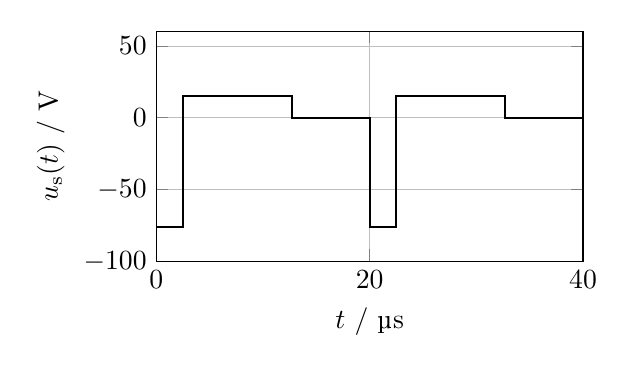
\begin{tikzpicture}
        \begin{axis}[
            width=7cm, height=4.5cm,
            grid=both,
            major grid style={line width=.2pt,draw=gray!50},
            minor grid style={line width=.1pt,draw=gray!20},
            xlabel={$t$ / µs},
            ylabel={$u_\mathrm{s}(t)$ / V},
           % title={$i_\mathrm{L}$ for minimum output power},
            xmin=0, xmax=40,
            ymin=-100, ymax=60,
            xtick={0, 20, 40},
            ytick={-100, -50, 0, 50},
            ]
            % Einschaltverhalten graph
            \addplot[
                thick,
                mark=none,
                color=black,
            ] coordinates {
                (0,0) (0,-76.4) (2.5,-76.4) (2.5, 15) (12.7, 15) (12.7, 0) (20, 0) (20, 0) (20, -76.4) (22.5, -76.4)(22.5, 15) (32.7, 15) (32.7, 0) (40, 0)
            };
        \end{axis}
        \end{tikzpicture} 
    \caption{Display of the voltage $u_\mathrm{T}(t)$ and $u_\mathrm{s}(t)$.}
    \label{fig:voltageTransistorPeriodTask1}

          
    \end{solutionfigure}